\chapter{Wnioski}

Po szczeg�owym przeanalizowaniu ka�dej metody na 7 sewencjach testowych mo�na doj�� do wniosku, i� �adnej z nich nie mo�na okre�li� mianem uniwersalnej - rezultaty zalez� od czynnik�w takich jak o�wietlenie, wyst�powanie cienia, dynamika sekwencji wideo, przej�cia tonalne element�w t�a. Dodatkowo, ka�da z metod posiada jeden lub kilka wsp�czynnik�w, kt�re nale�y dobra� indywidualnie dla ka�dej sekwencji (cz�sto metod� pr�b i b��d�w).  Z�y dob�r wspomnianych wsp�czynnik�w mo�e doprowadzi� do niepoprawnego zainicjalizowania t�a i powstania b��dnych modeli, jak na obrazach poni�ej:


\begin{figure}[H]
        \centering
        \begin{subfigure}[b]{0.3\textwidth}
                \centering
                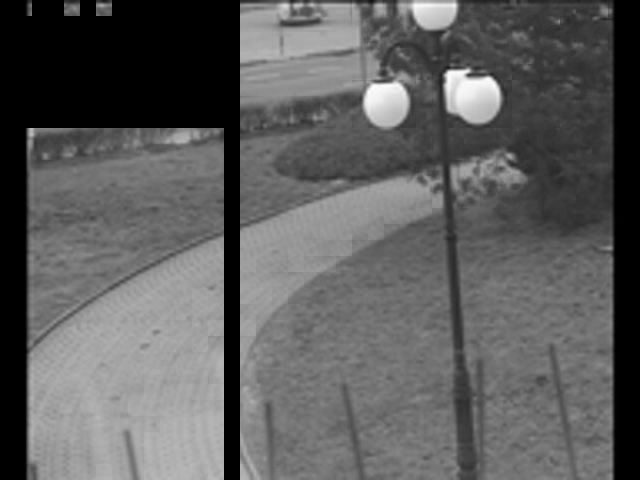
\includegraphics[width=\textwidth]{clip_02_broken.png}
                \centering
                \caption{$DCT\;T_{corr}=0.8$ $T_{MAD}=10$}
        \end{subfigure}
        \begin{subfigure}[b]{0.3\textwidth}
                \centering
                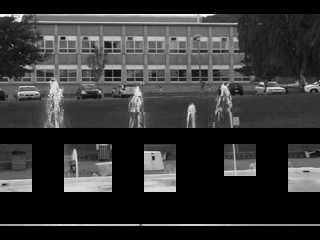
\includegraphics[width=\textwidth]{fountain_broken.png}
                \caption{$Hadamard\;T_{corr}=0.9$ $T_{MAD}=10$}        
                \end{subfigure}
        \begin{subfigure}[b]{0.3\textwidth}
                \centering
                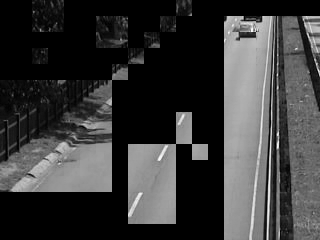
\includegraphics[width=\textwidth]{highway_broken.png}
                \caption{$DCT\;T_{corr}=0.9$ $T_{MAD}=10$}
        \end{subfigure}
        \caption{Obrazy wynikowe dla sekwencji clip\_03.mpg}
\end{figure}